\documentclass{article}
\usepackage{color}
\usepackage{url}
\usepackage{subfigure}
\usepackage{amsmath}
\usepackage{bm}
\usepackage{bbm}
\usepackage{amsfonts}
\usepackage{amssymb}
\usepackage{graphicx}
\usepackage[round]{natbib}

../../reproducible/tex/definitions.tex

\begin{document}

\section{Introduction}

Many systems biology models consist of interacting sets of
differential equations. Given full knowledge of the functions
involved in these systems traditional methods of systems
identification could be used to parameterize the models. A
particularly challenging aspect of biological systems is the
scarcity of the data. Some of the model components may be
unobservable, and those that are observed are not normally
sampled at a high rate, particularly not in the context of high
throughput experiments such as gene expression microarray and
RNA-sequencing. This
means that important sources of information are missing. In this
chapter we consider a two pronged approach to dealing with this
problem. In particular we look at modeling missing components of
the model through a basis function approximation to the functions
that can't be observed. We look at generalized linear models as a
potential approach to mapping these missing nonlinear
functions. Unfortunately, as the complexity of these models
increases, so does the number of parameters. We therefore
consider Bayesian approaches to dealing with the increasing
number of parameters. As we increase the complexity of the model
further, we find that these generalized linear models converge on
a particular probabilistic process known as a Gaussian process. We
then explore the use of Gaussian processes in biological modeling
with a particular focus on transcriptional networks and gene
expression data. We will review simple cascade models of
translation and transcription that can be used for genome-wide
target identification. We then introduce nonlinearities into the
differential equations. This means that we need to resort to
sampling methods, such as Markov chain Monte Carlo, to perform
inference in the systems. We briefly review an efficient approach
to sampling and demonstrate its use in modeling transcriptional
regulation.

\subsection{A Simple Systems Biology Model}

Gene expression is governed by transcription factors. To analyze
expression, we need to form a mathematical idealization of this
process. The exact mechanism behind transcription is not yet fully
understood, but a coarse mathematical representation of the system
would assume that the rate of production of a given gene's mRNA is
dependent on the amount of transcription factor in the cell. When
collating gene expression from many cells in a tissue we might model
the rate of mRNA production through an ordinary differential
equation. \cite{Barenco:ranked06} described just such a model of gene
expression,
\begin{equation}
\diff{\mrnaConcentration_j(t)}{t} = \basalRate_j + \sensitivity_j \tfConcentration(t) -\decayRate_j \mrnaConcentration_j(t), \label{eq:differentialEquation}
\end{equation}
where the rate of production of the $j$th gene's mRNA is dependent on
a basal rate of transcription, $\basalRate_j$, a sensitivity,
$\sensitivity_j$ to the governing transcription factor concentration,
$\tfConcentration(t)$ and a rate of decay, $\decayRate_j$. In this
simple model each of the genes is assumed to be governed by a
single input transcription factor and this is known as a single input
module motif \citep{Alon:systems06}. Short of assuming that the mRNA
concentration is linearly related to the transcription factor
concentration\footnote{This would be equivalent to assuming very high
  decay in the simple model we describe. Models like this
  are widely used. One can see clustering to find coregulated targets
  as making this assumption. The assumption is made more explicitly in
  some genomewide analysis models~\citep[e.g.][]{Sanguinetti:chipvar06,Sanguinetti:chipdyno06}.} this is
perhaps the simplest model of transcriptional regulation that can be
composed. It has a closed form solution for the mRNA concentration
that depends on the transcription factor (TF) concentration. If we assume that the system
starts at $t=0$ then we have
\begin{equation}
\mrnaConcentration_j(t) = a_je^{-\decayRate_{j}t} +
\frac{\basalRate_j}{\decayRate_j} +
\sensitivity_je^{-\decayRate_{j}t}\int_0^t
e^{\decayRate_{j}u}\tfConcentration(u) \mathrm{d}u 
\label{eq:differentialEquationSoln}
\end{equation}
where the initial value for the mRNA concentration is given by
$\mrnaConcentration_j(0)=\frac{\basalRate_j}{\decayRate_j}+a_j$.

The simple model described above can be extended through nonlinear
response, active degradation of the mRNA, stochastic effects, and so
on. However, it clearly illustrates the main issue we wish to address
in this chapter. Namely, how do we deal with the fact that the
transcription factor concentration, $\tfConcentration(t)$ may be
unobservable? 

Our preliminary studies in this area were inspired by the work of
\cite{Barenco:ranked06} who (ignoring the transient term) reordered
the equation so that for each observation time, $t_1, \dots,
t_\numData$, they had
\[
\tfConcentration(t_k) =
\sensitivity_j^{-1}\left(\diff{\mrnaConcentration_j(t_k)}{t} -
  \basalRate_j + \decayRate_j \mrnaConcentration_j(t_k)\right).
\]
They then created pseudo-observations of the production rates of the
mRNA, $\diff{\mrnaConcentration_j(t_i)}{t}$, through fitting
polynomials to their time series and computing gradients at each time
point. This gave them an estimate for the TF concentration and they
used Bayesian sampling to estimate the model parameters.

\cite{Khanin:repression06} considered a similar equation with a
nonlinear repression response. They and \cite{Rogers:model06b}, who
also considered single input motifs, dealt with the missing function
through fitting a piecewise constant approximation to the missing
function. In this chapter our focus will be on an alternative
approach: modeling the missing function with a generalized linear
model.

\section{Generalized Linear Model}

For our purposes a generalized linear model can be seen as
constructing a function through a weighted sum of
nonlinearities. Formally, we assume that a function, $f(t)$ can be
represented as
\[
f(t) = \sum_{k=1}^\numBasisFunc \weightScalar_k\basisFunc_k(t),
\]
where the basis function has a nonlinear form. One possibility is a basis derived from a Gaussian form,
\begin{equation}
\basisFunc_k(t) = \frac{1}{\sqrt{\pi\lengthScale_k^2}}\exp\left(-\frac{(t-\tau_k)^2}{\lengthScale{}_k^2}\right). \label{eq:eqBasis}
\end{equation}
Here $\tau_k$ represents a location parameter which gives the center
of the basis function and $\lengthScale$ represents a timescale
parameter which gives the width of the basis function (or the
timescale over which it is active). As the distance between $t$ and
$\tau_k$ increases the basis function approaches zero. This is
therefore sometimes described as a ``local'' basis function. In
\reffig{fig:basisFunctions} we show a set of bases and some nonlinear
functions that can be derived from them using different weights.
\begin{figure}
  \begin{center}
    \subfigure[Set of three basis functions.]{
      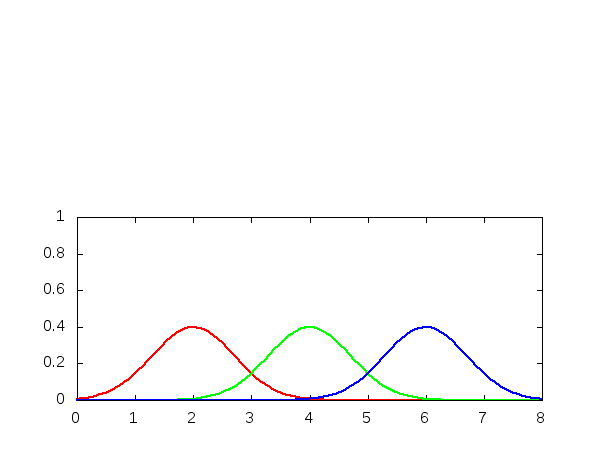
\includegraphics[width=0.6\textwidth]{../../../gpsim/tex/diagrams/demBasisSample0}}
    \subfigure[Linear combination of basis with $\weightScalar_1=0.875$, $\weightScalar_2=-0.388$, and $\weightScalar_3=-2.01$.]{
      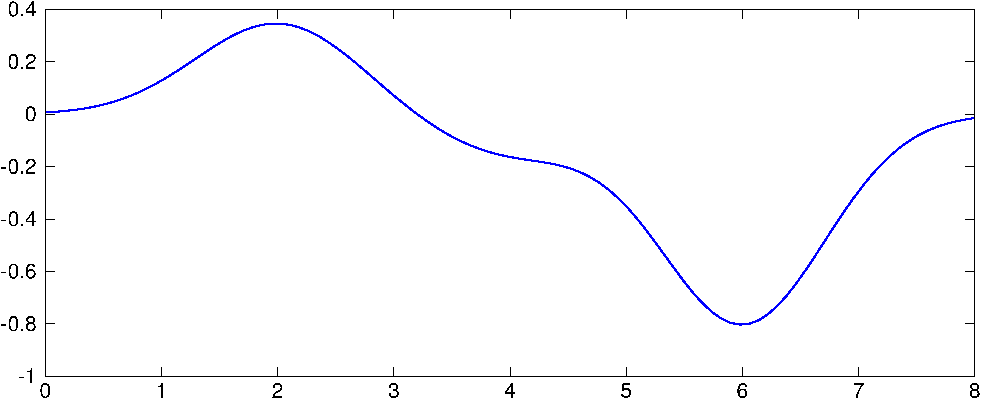
\includegraphics[width=0.6\textwidth]{../../../gpsim/tex/diagrams/demBasisSample1}}
    \subfigure[Linear combination of basis with $\weightScalar_1=-0.359$, $\weightScalar_2=1.23$, and $\weightScalar_3=-0.328$.]{
      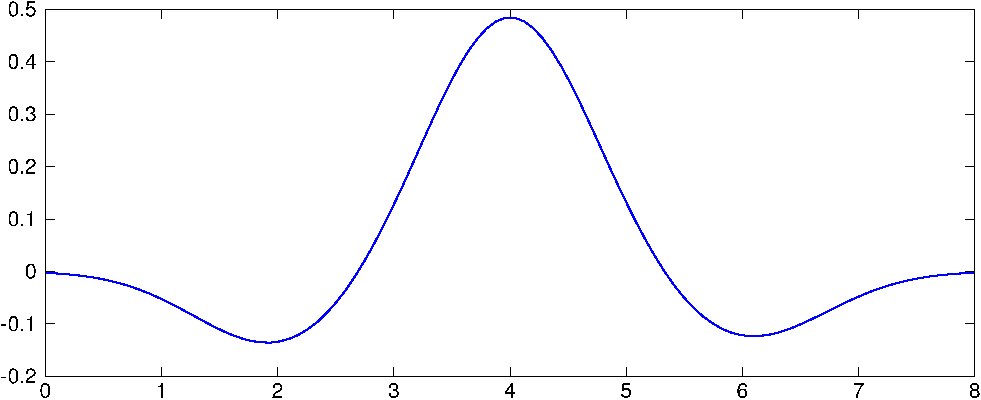
\includegraphics[width=0.6\textwidth]{../../../gpsim/tex/diagrams/demBasisSample2}}
    \subfigure[Linear combination of basis with $\weightScalar_1=-1.56$, $\weightScalar_2=-0.74$, and $\weightScalar_3=1.69$.]{
      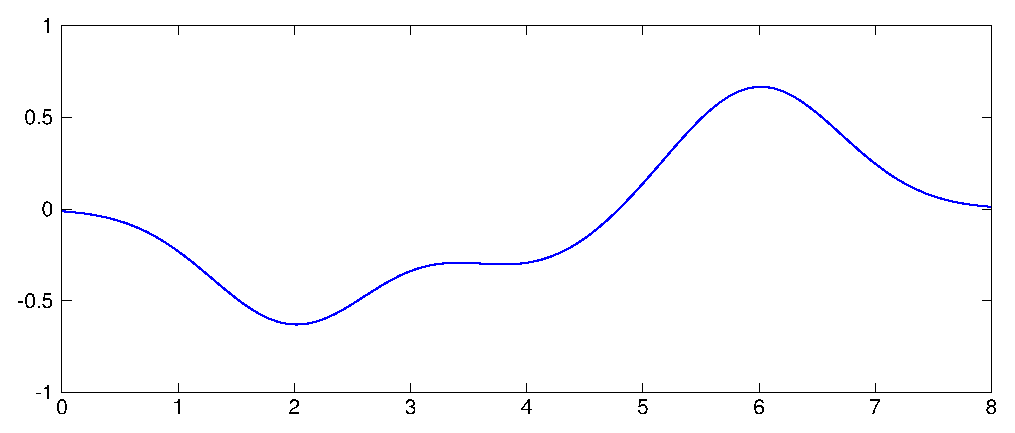
\includegraphics[width=0.6\textwidth]{../../../gpsim/tex/diagrams/demBasisSample3}}
  \end{center}

  \caption{Some functions based on a simple basis set with three
    members. Location parameters of the basis functions are set to
    $\tau_k = 2, 4, 6$ and the time scale of the bases is set to
    1. Functions derived from these bases are shown for different
    weights. Each weight was sampled from a standard normal
    density.}\label{fig:basisFunctions}
\end{figure}

Our aim is to introduce this representation of the function into our
model of the system. We assume that the transcription factor
concentration can be represented through basis functions so we have,
\[
\tfConcentration(t) = \sum_{k=1}^\numBasisFunc \weightScalar_k\basisFunc_k(t).
\]
Taking the simple linear differential equation model given in
\refeq{eq:differentialEquation} we can substitute in our
representation of the transcription factor concentration and recover
\[
\diff{\mrnaConcentration_j(t)}{t} = \basalRate_j + \sensitivity_j \sum_{k=1}^\numBasisFunc \weightScalar_k \basisFunc_k(t) -\decayRate_j \mrnaConcentration_j(t). 
\]
Substituting this into the solution for $m_j(t)$ we have
\begin{equation}
\mrnaConcentration_j(t) = a_je^{-\decayRate_{j}t} + \frac{\basalRate_j}{\decayRate_j} + \sensitivity_j\sum_{k=1}^\numBasisFunc \weightScalar_k e^{-\decayRate_{j}t}\int_0^t e^{\decayRate_{j}u} \basisFunc_k(u) \mathrm{d}u \label{eq:basisFunctionSolution}
\end{equation}
%\[
%\int_0^t \exp\left(\left(\decayRate_j+2\frac{\tau_k}{\lengthScale^2}\right)u-\frac{u^2}{\lengthScale^2} -\frac{\tau_k^2}{\lengthScale^2}\right)\mathrm{d}u
%\]
%\[
%\int_0^t \exp\left( -\frac{\left(u-\frac{\decayRate_j\lengthScale^2}{2}-\tau_k\right)^2}{\lengthScale^2}  -\frac{\tau_k^2}{\lengthScale^2} + \frac{\left(\frac{\decayRate_j\lengthScale^2}{2} + \tau_k\right)^2}{\lengthScale^2}\right)\mathrm{d}u
%\]
%\[
%\int_0^t \exp\left( -\frac{\left(u-\frac{\decayRate_j\lengthScale^2}{2}-\tau_k\right)^2}{\lengthScale^2}  + \decayRate_j\tau_k + \frac{\decayRate_j^2\lengthScale^2}{4} \right)\mathrm{d}u
%\]
where we have been able to pull the weighted sum over the basis
functions outside the integral. Our solution for the mRNA
concentration is now also expressed as a generalized linear model. Now
the basis set consists of a transient term, $a_je^{-\decayRate_jt}$, a
constant term, $\frac{\basalRate_j}{\decayRate_j}$, and a weighted sum
of convolutions of our original basis. For some choices for
$\basisFunc_k(t)$ the integral in \refeq{eq:basisFunctionSolution}
will be tractable. In particular if we use the Gaussian form shown in
\refeq{eq:eqBasis} we can show that,
 \begin{align*}
 e^{-\decayRate_{j}t}\int_0^t e^{\decayRate_{j}u} \basisFunc_k(u) \mathrm{d}u =& e^{-\decayRate_j(t-\tau_k)}e^{\frac{\decayRate_j^2\lengthScale{}_k^2}{4}}
\frac{1}{2}\bigg[\erf\left(\frac{t-\left(\tau_k+\frac{\decayRate_j\lengthScale{}_k^2}{2}\right)}{\lengthScale_k}\right)\\&-\erf\left(-\frac{\tau_k+\frac{\decayRate_j\lengthScale{}_k^2}{2}}{\lengthScale_k}\right)\bigg]
\end{align*}
where $\erf(\cdot)$ is the error function defined as
\[
\erf(x) = \int_{0}^x \frac{2}{\sqrt{\pi}}\exp\left(-z^2\right) \mathrm{d}z.
\]
For fixed parameters, $a_j$, $\sensitivity_j$, $\decayRate_j$,
$\basalRate_j$ there is a deterministic relationship between the
output mRNA concentration, $\mrnaConcentration_j(t)$ and a governing
TF concentration, $\tfConcentration(t)$. In
\reffig{fig:convolvedBasisFunctions} we show functions that correspond
to high, medium and low decay rates that result from solving the
differential equation for the different TF concentrations shown in
\reffig{fig:basisFunctions}.
\begin{figure}
  \begin{center}
    \subfigure[Three basis functions after convolution. \emph{Left}: $\decayRate_1=0.01$, \emph{middle}: $\decayRate_2=0.1$, \emph{right} $\decayRate_3=1$]{
      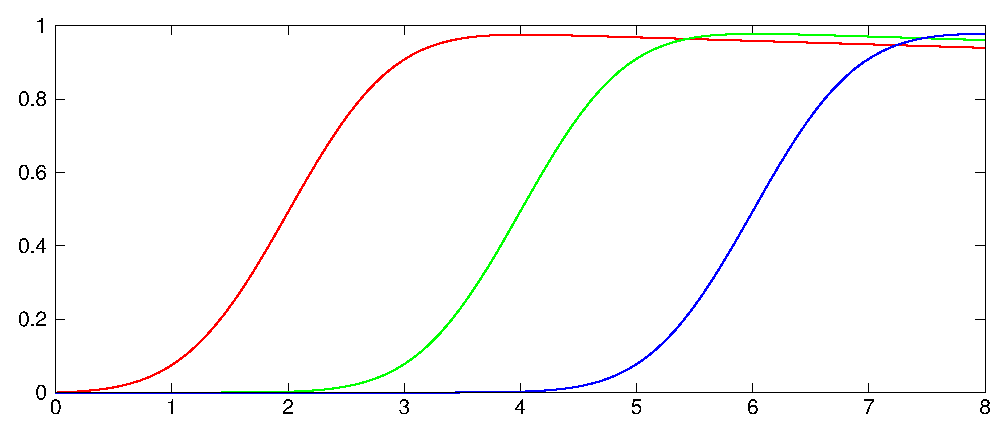
\includegraphics[width=0.3\textwidth]{../../../gpsim/tex/diagrams/demBasisSample0_1}\hfill
      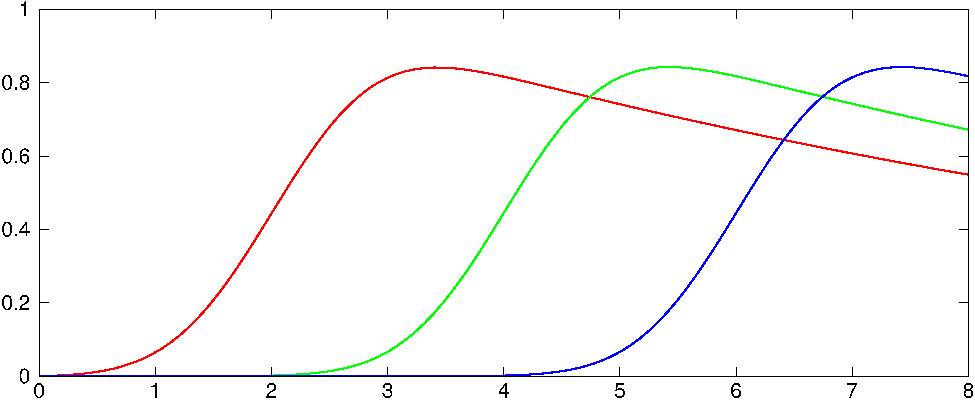
\includegraphics[width=0.3\textwidth]{../../../gpsim/tex/diagrams/demBasisSample0_2}\hfill      
      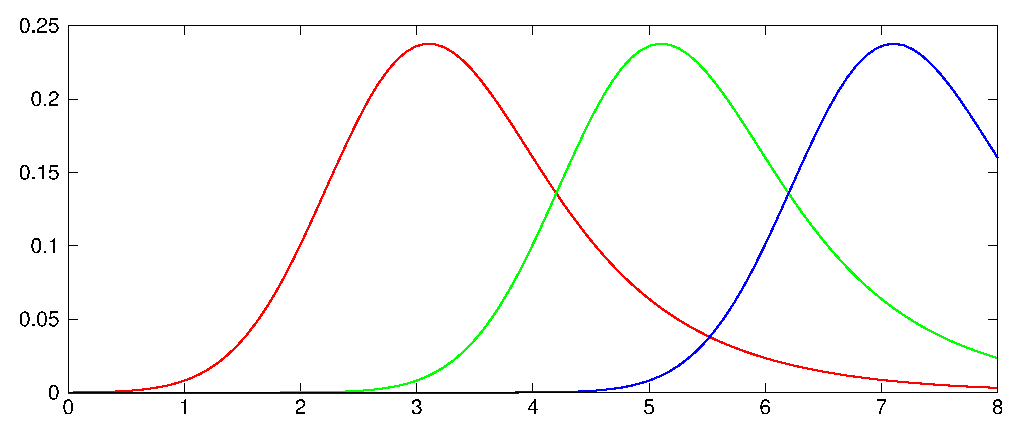
\includegraphics[width=0.3\textwidth]{../../../gpsim/tex/diagrams/demBasisSample0_3}}
    \subfigure[Linear combination of convolved basis with $\weightScalar_1=0.875$, $\weightScalar_2=-0.388$, and $\weightScalar_3=-2.01$.]{
      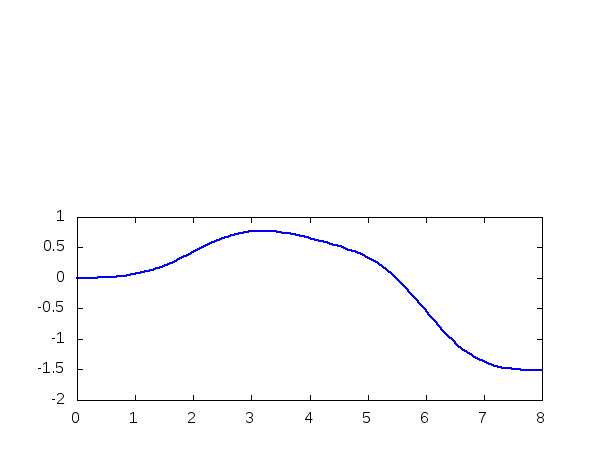
\includegraphics[width=0.3\textwidth]{../../../gpsim/tex/diagrams/demBasisSample1_1}\hfill
      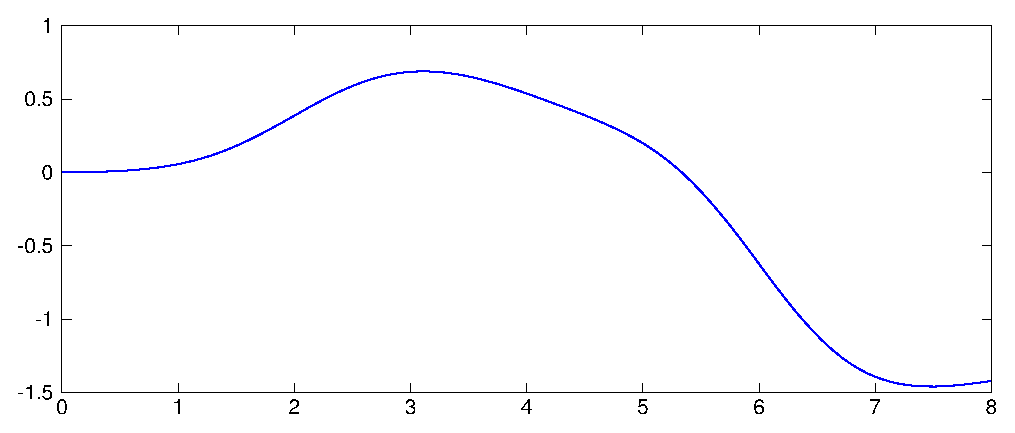
\includegraphics[width=0.3\textwidth]{../../../gpsim/tex/diagrams/demBasisSample1_2}\hfill      
      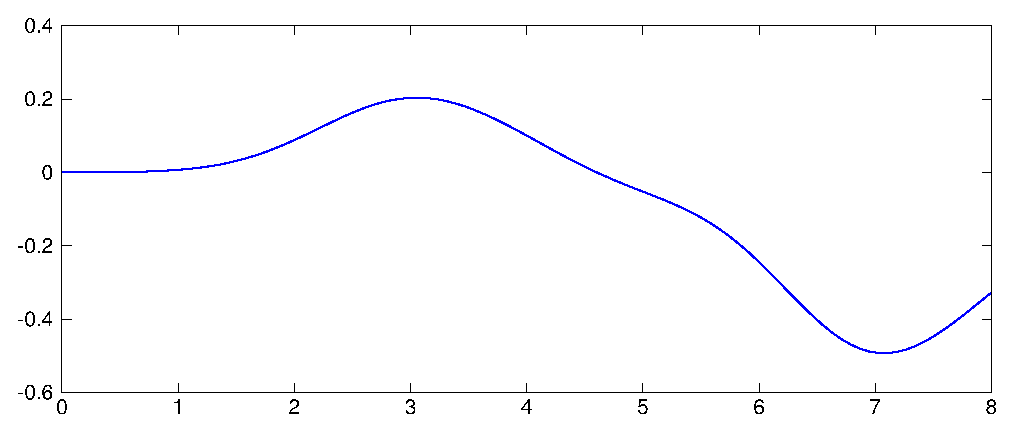
\includegraphics[width=0.3\textwidth]{../../../gpsim/tex/diagrams/demBasisSample1_3}}
    \subfigure[Linear combination of convolved basis with $\weightScalar_1=-0.359$, $\weightScalar_2=1.23$, and $\weightScalar_3=-0.328$.]{
      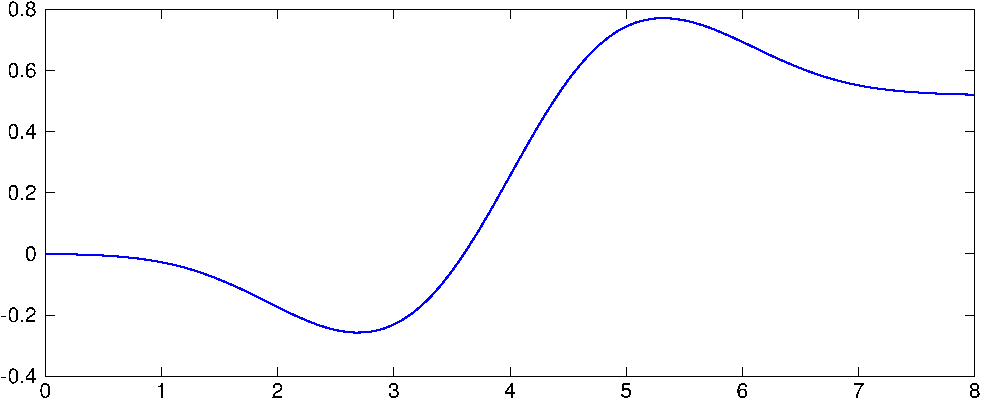
\includegraphics[width=0.3\textwidth]{../../../gpsim/tex/diagrams/demBasisSample2_1}\hfill
      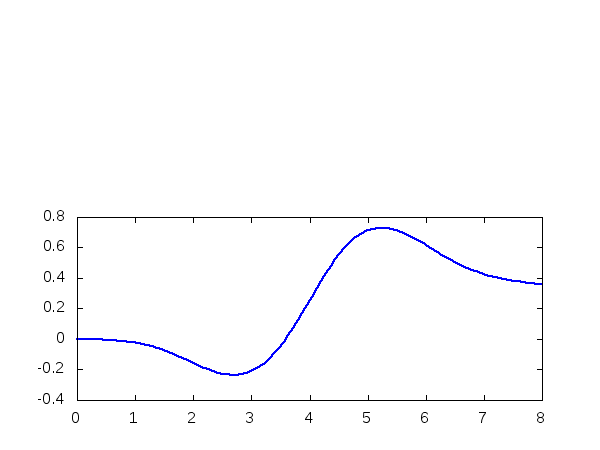
\includegraphics[width=0.3\textwidth]{../../../gpsim/tex/diagrams/demBasisSample2_2}\hfill      
      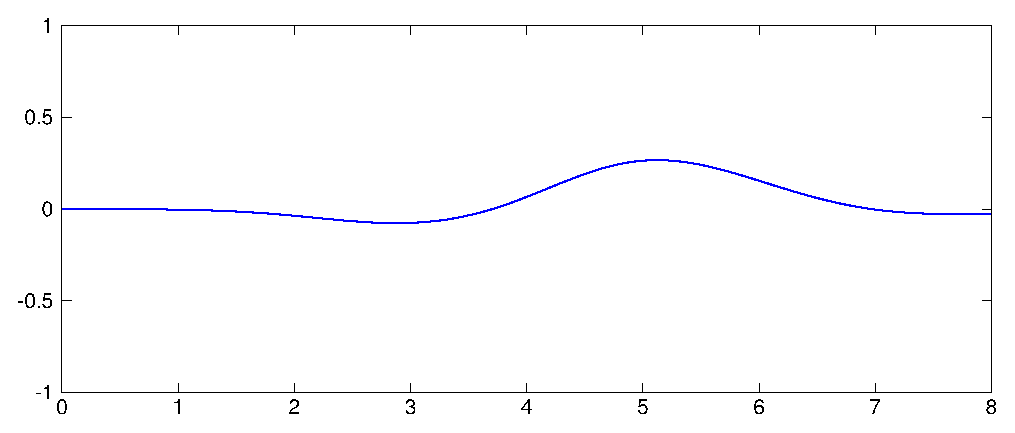
\includegraphics[width=0.3\textwidth]{../../../gpsim/tex/diagrams/demBasisSample2_3}}
    \subfigure[Linear combination of convolved basis with $\weightScalar_1=-1.56$, $\weightScalar_2=-0.74$, and $\weightScalar_3=1.69$.]{
      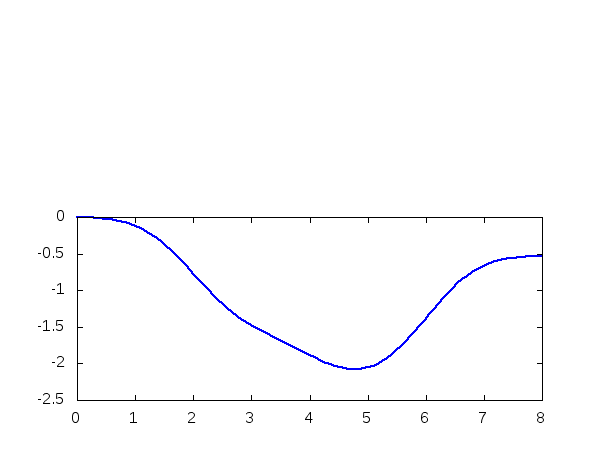
\includegraphics[width=0.3\textwidth]{../../../gpsim/tex/diagrams/demBasisSample3_1}\hfill
      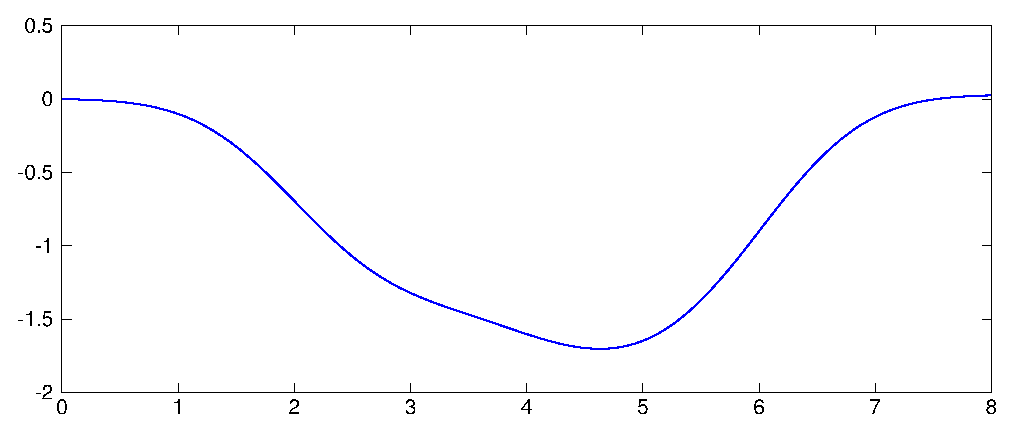
\includegraphics[width=0.3\textwidth]{../../../gpsim/tex/diagrams/demBasisSample3_2}\hfill      
      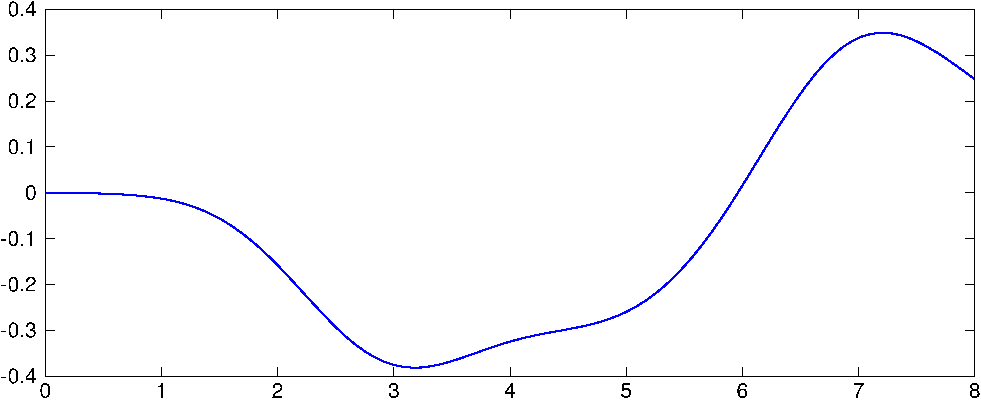
\includegraphics[width=0.3\textwidth]{../../../gpsim/tex/diagrams/demBasisSample3_3}}
  \end{center}

  \caption{The bases in \reffig{fig:basisFunctions} have been pushed
    through the differential equation to give the convolved basis
    shown in (a). We took $a_j=0$, $\basalRate_j=0$ and
    $\sensitivity_j=1$ for $j=1, 2, 3$. Decays were then set to be
    low, $\decayRate_1=0.01$, medium, $\decayRate_2=0.1$, and high,
    $\decayRate_3=1$. in (b)-(d) we see mRNA concentrations derived
    from these bases with different weights,
    $\weightScalar_k$. Weights match those shown in
    \reffig{fig:basisFunctions}. In each row the leftmost plot is the
    result of convolving with a low decay rate ($\decayRate_1=0.01$),
    the middle plot a medium decay rate ($\decayRate_2=0.1$) and the
    rightmost a higher decay rate
    ($\decayRate_3=1$).}\label{fig:convolvedBasisFunctions}

\end{figure}
By setting $\left\{a_j, \basalRate_j\right\}_{j=1}^3$ to zero and
$\left\{\sensitivity_j\right\}_{j=1}^3$ to one we ensure that the
differences between all the solutions are arising only from the
different responses to the underlying basis from
\reffig{fig:basisFunctions}. The solution for each individual basis
function is shown in the top row of
\reffig{fig:convolvedBasisFunctions}. The solution for each different set of weights from \reffig{fig:basisFunctions} is then simply the weighted sum of the relevant weights multiplied by the convolved basis functions.

\subsection{Fitting Basis Function Models}

Given a basis set, $\left\{\phi_k(t)\right\}_{k=1}^\numBasisFunc$, a
set of weights, $\left\{\weightScalar_k\right\}_{k=1}^\numBasisFunc$,
and the parameters of the differential equation, $\{\basalRate_j,
\decayRate_j, \sensitivity_j\}_{j=1}^\dataDim$, we can solve the
differential equations for the mRNA concentrations,
$\left\{\mrnaConcentration_j(t)\right\}_{j=1}^\dataDim$. We can
determine all these parameters of the model (including the parameters
of the basis functions) by fitting through maximum likelihood. If we
assume Gaussian noise of variance $\dataStd^2$ we can compute the log
likelihood of an observed data set of mRNA concentrations, perhaps
obtained from a gene expression microarray,
\[
\log p(\dataMatrix|\weightVector) = -\frac{\dataDim}{2}\log 2\pi\dataStd^2 -\frac{1}{2\dataStd^2}\sum_{j=1}^\dataDim \sum_{i=1}^\numData(\mrnaConcentration_j(t_i) - y_{i,j})^2,
\]
where the gene expression data has been collected at times
$\left\{t_i\right\}$ and has values given by $\left\{y_{i,j}\right\}$
for the $j$th gene. We have used the notation
$\mrnaConcentration_j(t_i)$ to denote the value of the predicted mRNA
concentration for the $j$th gene at the $i$th time point. Bearing in
mind that this is dependent on the parameters of the $j$th
differential equation and the basis functions, we can maximize this
log likelihood with respect to all these parameters and the noise
variance. Here, in our representation of the likelihood $p(\dataMatrix|\weightVector)$, we have only made explicit the conditioning on the vector of weights,  $\weightVector=\left[\weightScalar_1,\dots,\weightScalar_\numBasisFunc\right]^\top$, as we will mainly focus on maximization with respect to this vector. With such a probabilistic formulation we can also exploit
the PUMA \citep{Milo:probabilistic03,Liu:tractable04} framework for
propagating uncertainty through microarray analysis and associate an
individual variance $\dataStd_{i,j}$ with each gene expression
observation, $y_{i,j}$. 

Working with the convolved basis set we have
\[
\phi^\prime_{j,k}(t) = \sensitivity_je^{-\decayRate_{j}t}\int_0^t
e^{\decayRate_{j}u} \basisFunc_k(u) \mathrm{d}u.
\]
We can then write a particular mRNA concentration as
\[
\mrnaConcentration_j(t) = a_ie^{-\decayRate_j t} + \frac{\basalRate_j}{\decayRate_j} + \weightVector^\top \basisFuncVector^\prime_{j}(t)
\]
where $\weightVector$ is a vector of the values
$\{\weightScalar_k\}_{k=1}^\numBasisFunc$ and
$\basisFuncVector^\prime(t)$ is a vector valued function representing
the values of the basis functions
$\left\{\basisFunc^\prime_{j,k}(t)\right\}_{k=1}^\numBasisFunc$. Ignoring the basal rate and $a_i$ for the moment, we can write the log likelihood as
\begin{align*}
p(\dataMatrix|\weightVector) =& -\frac{\dataDim}{2}\log 2\pi\dataStd^2\\
& -\frac{1}{2\dataStd^2}\left(-\weightVector^\top\sum_{j=1}^\dataDim \sum_{i=1}^\numData\basisFuncVector^\prime_j(t_i)\basisFuncVector^\prime_j(t_i)^\top\weightVector
+2\sum_{j=1}^\dataDim \sum_{i=1}^\numData\weightVector^\top\basisFuncVector^\prime_j(t_i)y_{i,j} + y_{i,j}^2\right)
\end{align*}
which can be maximized with respect to $\weightVector$ by finding a stationary point of the log likelihood,
\[
\weightVector = \left[\sum_{j=1}^\dataDim \sum_{i=1}^\numData\basisFuncVector^\prime_j(t_i)\basisFuncVector^\prime_j(t_i)^\top\right]^{-1}\sum_{j=1}^\dataDim \sum_{i=1}^\numData\basisFuncVector^\prime_j(t_i)y_{i,j}.
\]
If we require a lot of flexibility for our model of the TF
concentration, $\tfConcentration(t)$, we can use a large number of
basis functions, $\numBasisFunc$. However, as we increase the number
of basis functions we may find that we are no longer able to compute
the maximum likelihood solution for $\weightVector$. If
$\numBasisFunc>\numData\dataDim$ then the matrix given by
$\sum_{j=1}^\dataDim
\sum_{i=1}^\numData\basisFuncVector^\prime_j(t_i)\basisFuncVector^\prime_j(t_i)^\top$
will not be invertible. A solution to this problem is to handle
$\weightVector$ through Bayesian inference (see
\citet{Lawrence:licsbbayes10} for a brief introduction). In Bayesian
inference, parameters are treated with a prior distribution, in this
case $p(\weightVector)$, and rather than being maximized they are
integrated out:
\[
p(\dataMatrix) =\int p(\dataMatrix|\weightVector)p(\weightVector)\mathrm{d}\weightVector.
\]
The quantity $p(\dataMatrix)$ is called the marginal likelihood,
integrated likelihood or evidence of the model, which is important for
model comparison~\citep{MacKay:information03}.
% a posterior distribution for the weights can the be computed as
% \[
% p(\weightVector|\dataMatrix) = \frac{p(\dataMatrix|\weightVector)p(\weightVector)}{p(\dataMatrix)}
% \]
% this is known as Bayes' rule.
If we place a zero mean Gaussian prior density over $\weightVector$,
\[
p(\weightVector)=\frac{1}{\sqrt{2\pi}\det{\covarianceMatrix}^{\frac{1}{2}}}\exp\left(-\frac{1}{2}\weightVector^\top \covarianceMatrix^{-1}\weightVector\right)
\]
we can compute the marginal likelihood of the data analytically and we
find that it is
given by
\[
p(\dataMatrix) = \frac{1}{\sqrt{2\pi}\det{\kernelMatrix + \dataStd^2\eye}^\frac{1}{2}}\exp\left(-\frac{1}{2}\dataVector^\top \left(\kernelMatrix + \dataStd^2\eye\right)^{-1}\dataVector\right),
\]
where $\dataVector$ is a ``stacked'' version of the data matrix,
i.e. it is composed of the columns from $\dataMatrix$ stacked on top
of one another. The matrix $\kernelMatrix$ gives the covariance
between the different mRNA concentrations at different times. It is
structured as a block matrix with $\dataDim\times\dataDim$ blocks,
each block of size $\numData\times\numData$. The diagonal blocks give
covariances of a single gene output, while off-diagonal blocks give
\emph{cross covariances} between different outputs. In general we can define
each element of $\kernelMatrix$ to be $\kernel_{i,j}(t, t^\prime) =
\basisFuncVector^\prime_i(t)^\top\covarianceMatrix\basisFuncVector^\prime_j(t')$. This
denotes the covariance between the $i$ and $j$th mRNA concentrations
computed between times $t$ and $t^\prime$. % We can depict the structure
% of this covariance function using a color map to represent the
% function values as shown in \reffig{fig:covarianceStructure}.
% \begin{figure}

%   \caption{Structure of $\kernelMatrix$ from the marginal likelihood's
%     covariance matrix.}\label{fig:covarianceStructure}
% \end{figure}

\subsubsection{Relationship with Basis of $\tfConcentration(t)$}

The model as we described is dependent on our choice of basis function
for $\tfConcentration(t)$. An interesting feature is that we can
represent all the elements of the marginal likelihood's covariance matrix through
the inner product of the basis, $\kernel_{0,0}(t,
t^\prime)=\basisFuncVector(t)^\top\covarianceMatrix\basisFuncVector(t^\prime)$:
\begin{equation}
  \label{eq:convolution}
\kernel_{i,j}(t,t^\prime) = \sensitivity_j\sensitivity_i e^{-\decayRate_{i}t-\decayRate_{j}t^\prime}\int_0^t
e^{\decayRate_{i}u} \int_0^{t^\prime} e^{\decayRate_{j}u^\prime}\underbrace{\basisFuncVector(u)^\top \covarianceMatrix \basisFuncVector(u^\prime)}_{\kernel_{0,0}(u, u^\prime)}\mathrm{d}u^\prime \mathrm{d}u.
\end{equation}
In fact this equation holds in general: as long as $k_{0,0}(t,
t^\prime)$ is a positive definite function, it represents an inner
product of a basis set. If we consider a spherical prior for
$\weightVector$, so $\covarianceMatrix=\gamma\eye$, then we can write
$\kernel_{0,0}(t,t^\prime) = \gamma
\basisFuncVector(t)^\top\basisFuncVector(t^\prime)$. Now, instead of maximizing
over all different weight parameters, $\weightVector$, we only need to
find $\gamma$. Through marginalization we have reduced the number of
parameters in the system by $\numBasisFunc-1$. A problem remains
though, each basis function has a center, $\tau_k$, and these
locations represent an additional $\numBasisFunc$ parameters that also
need to be determined. We now show how these parameters can also be
eliminated. We will consider a limit that allows us to
effectively take the number of basis functions, $\numBasisFunc\rightarrow\infty$.

\subsection{An Infinite Basis}

Now we have eliminated the parameters $\weightVector$ we are left to
decide the number of basis functions, $\numBasisFunc$, and the location of these basis
functions, $\left\{\tau_k\right\}_{k=1}^\numBasisFunc$. First we will explore what happens when we place those basis
functions at uniform intervals over time so we have
\[
\tfConcentration(t) = \sum_{k=1}^\numBasisFunc \weightScalar_k \frac{1}{\sqrt{\pi\lengthScale{}^2}}\exp\left(-\frac{(t-a -\Delta\tau \cdot k)^2}{\lengthScale{}^2}\right),
\]
where we have set the location parameter of each $\basisFunc_k(t)$ to
\[
\tau_k = a+\Delta\tau\cdot k.
\]
We showed that the marginal likelihood of the model is entirely
dependent on the inner product between basis vectors at different
times. For the basis at uniform intervals this can be written as
% \[
% \kernel_{0,0}\left(t,t^\prime\right) = \frac{\gamma}{2\pi\lengthScale{}^2}\sum_{k=1}^{\numBasisFunc} \exp\left(
%   -\frac{t^2 + \left.t^\prime\right.^2 - 2\tau_k \left(t+t^\prime\right) +
%     2\tau_k^2}{2\lengthScale{}^2} \right),
% \]
% we can specify the bases in terms of their indices,
\[
\kernel_{0,0}\left(t,t^\prime\right) = \frac{\gamma}{\pi
  \lengthScale^2}\sum_{k=1}^{\numBasisFunc} \exp\left( -\frac{t^2 +
    \left.t^\prime\right.^2 - 2\left(a+\Delta\tau\cdot k\right)
    \left(t+t^\prime\right) + 2\left(a+\Delta\tau \cdot k\right)^2}{
    \lengthScale{}^2} \right).
\]
More basis functions allow greater flexibility in our model of the TF
concentration. We can increase the number of basis functions we use in
the interval between $a$ and $b$ by decreasing the interval
$\Delta\tau$. However, to do this without increasing the expected
variance of the resulting TF concentration we need to scale down the
variance of the prior distribution for $\weightVector$. This can be
done by setting the variance parameter to be proportional to the
interval, so we take $\gamma = \alpha\Delta\tau$. Now we have basis
functions where the location of the leftmost basis function, $k=1$, is
$\tau_1=a+\Delta\tau$ and the rightmost basis is
$\tau_\numBasisFunc=b$ so that $b= a+
\Delta\tau\cdot\numBasisFunc$. The fixed interval distance between $a$
and $b$ is therefore given by $b-a=(\numBasisFunc-1)\Delta \tau$.

We are going to increase the number of basis functions by taking the
limit as $\Delta \tau\rightarrow 0$. This will take us from a discrete
system to a continuous system. In this limit the number of basis
functions becomes infinite because we have $\numBasisFunc
=\lim_{\Delta \tau \rightarrow 0} \frac{b-a}{\Delta \tau} + 1$. In
other words we are moving from a fixed number of basis functions to
infinite basis functions. The inner product between the basis
functions becomes

\[
\kernel_{0,0}\left(t,t^\prime\right) = \frac{\alpha}{\pi \lengthScale^2}
\int_a^b \exp\left( -\frac{t^2 + \left.t^\prime\right.^2 - 2\tau
    \left(t+t^\prime\right) + 2\tau^2}{\lengthScale{}^2}
\right)\mathrm{d}\tau.
\]
Completing the square gives
\[
\kernel_{0,0}\left(t,t^\prime\right) = \frac{\alpha}{\pi \lengthScale^2}
\int_a^b \exp\left( -\frac{t^2 + \left.t^\prime\right.^2 + 2\left(\tau
      - \frac{1}{2}\left(t + t^\prime\right)\right)^2
    -\frac{1}{2}\left(t + t^\prime\right)^2}{\lengthScale{}^2}
\right)\mathrm{d}\tau
\]


\[
\kernel_{0,0}\left(t,t^\prime\right) =
\frac{\alpha}{\sqrt{2\pi\lengthScale{}^2}} \exp\left(
  -\frac{(t-t^\prime)^2}{2\lengthScale{}^2}\right) \sqrt{\frac{2}{\pi
    \lengthScale{}^2}}\int_a^b
\exp\left(-\frac{2}{\lengthScale^2}\left(\tau - \frac{t +
      t^\prime}{2}\right)^2 \right)\mathrm{d}\tau,
\]
\[
\kernel_{0,0}\left(t,t^\prime\right) =
\frac{\alpha}{\sqrt{2\pi\lengthScale{}^2}} \exp\left(
  -\frac{(t-t^\prime)^2}{2\lengthScale{}^2}\right)
\frac{1}{2}\left[1+\mathrm{erf}\left(\sqrt{\frac{2}{\lengthScale^2}}\left(\tau
      - \frac{t + t^\prime}{2}\right) \right)\right]_a^b,
\]
Performing the integration leads to 
\begin{align*}
\kernel_{0,0}\left(t,t^\prime\right) = &
\frac{\alpha}{\sqrt{2\pi\lengthScale{}^2}} \exp\left(
  -\frac{\left(t-t^\prime\right)^2}{2\lengthScale{}^2}\right)
\frac{1}{2}\bigg[\mathrm{erf}\left(\sqrt{\frac{2}{\lengthScale^2}}\left(b
      - \frac{t + t^\prime}{2}\right) \right) \\ & -
  \mathrm{erf}\left(\sqrt{\frac{2}{\lengthScale^2}}\left(a - \frac{t +
        t^\prime}{2}\right) \right)\bigg],
\end{align*}
Finally, if we take the limit as $a\rightarrow -\infty$ and
$b\rightarrow \infty$ (i.e. we have infinite basis functions
distributed across the entire real line) then the square bracketed
term on the right becomes 2 and we have

\begin{equation}
\kernel_{0,0}\left(t,t^\prime\right) =
\frac{\alpha}{\sqrt{2\pi\lengthScale^2}}\exp\left(
  -\frac{\left(t-t^\prime\right)^2}{2\lengthScale{}^2}\right),
  % Neil: What is this doing here: -AH
  % \\lengthScale ,
\label{eq:RBF}
\end{equation}
which is known as the squared exponential covariance function (despite the fact that it is not a squared exponential, but an exponentiated quadratic). 

The analysis above shows that if we take a one dimensional fixed
basis function model, we can increase the number of basis functions to
infinity and distribute them evenly across the real line. In this way
we loose the requirement to specify $\numBasisFunc$ location
parameters and further reduce the number of parameters in the
system. Without the Bayesian approach we had $2(\numBasisFunc +1) +
4\dataDim$ parameters. The combination of the Bayesian approach and
the use of infinite basis functions leads to $4\dataDim + 3$
parameters without any loss of model flexibility. In fact the resulting
model is more flexible as it is allowing for infinite basis
functions. Instead of specifying the basis function directly, we now
specify the covariance of the marginal through a positive definite
function $\kernel_{0,0}(t, t^\prime)$.

The procedure for moving from inner products,
$\basisFuncVector(t)^\top\basisFuncVector(t^\prime)$, to covariance functions,
$\kernel_{0,0}(t, t^\prime)$, is sometimes known as kernelization
\citep{Scholkopf:learning01} due to the fact that the covariance
function has the properties of a Mercer kernel. A function of two variables can be seen as a Mercer kernel when a
symmetric matrix of values from $\kernel_{0,0}(t, t^\prime)$ computed
for a vector of times $\mathbf{t}$ is always positive
semi-definite. In other words if $\kernel_{i,j} = \kernel_{0,0}(t_i,
t_j)$ is the element from the $i$th row and $j$th column of
$\kernelMatrix_{0,0}$ and $t_i$ is the $i$th element from $\mathbf{t}$, we
should have that $\kernelMatrix_{0,0}$ is a positive definite matrix for any
vector of inputs $\mathbf{t}$. This same property is what allows it to
be used as a covariance function: covariances must be positive
definite. The matrix $\kernelMatrix_{0,0}$ specifies the covariance between
instantiations of the function $\tfConcentration(t)$ at the times
given by $\mathbf{t}$. Mercer's theorem says that underlying all such
positive definite functions there is always a (possibly infinite)
feature space, $\basisFunc(t)$, which can be used to construct the
covariance function. For our example the relationship between the
feature space and this covariance function emerges naturally through
considering a Bayesian approach to a fixed basis function model. The
resulting model is known as a Gaussian process
\citep{Ohagan:curve78}. This perspective of converting from a
parametric model to a covariance function is one way of introducing
Gaussian processes (see also \citet{Williams:Gaussian95} and
\citet{Rasmussen:book06}). For an alternative introduction which
ignores the parametric interpretation see
\citet{Lawrence:licsbgp10}. 

%Finally, note that we can also construct
%networks with infinite basis functions through considering a Bayesian
%approach to the parameters of a non-linear model
%\citep{Williams:computation98}.

\subsection{Gaussian Processes}

Using the marginal likelihood of the model we described instead of the
model parameterized by $\weightVector$ can be understood as taking a
Gaussian process perspective on the model for
$\tfConcentration(t)$. Gaussian processes are powerful models for
nonlinear functions. They allow us to specify the characteristics of a
function through specifying its covariance function. Given a covariance function for the Gaussian process over $\tfConcentration$, the covariances between the target genes can also be computed from \refeq{eq:convolution}. Substituting $\kernel_{0,0}(t, t^\prime)=\basisFuncVector(t)^\top \covarianceMatrix \basisFuncVector(t^\prime)$ we have 
\[
\kernel_{i,j}(t,t^\prime) = \sensitivity_j\sensitivity_i e^{-\decayRate_{i}t-\decayRate_{j}t^\prime}\int_0^t
e^{\decayRate_{i}u} \int_0^{t^\prime} e^{\decayRate_{j}u^\prime}\kernel_{0,0}(u, u^\prime)\mathrm{d}u^\prime \mathrm{d}u.
\]
We can also compute the cross covariance between $\tfConcentration(t)$ and the $i$th output gene, 
\[
\kernel_{0,i}(t, t^\prime) = \sensitivity_i e^{-\decayRate_{i}t}\int_0^t
e^{\decayRate_{i}u} \kernel_{0,0}(u, t^\prime)\mathrm{d}u.
\]
This arises in the joint distribution of $\tfConcentration(t)$ and $\left\{\mrnaConcentration_i(t)\right\}_{i=1}^\dataDim$ which is also Gaussian with covariance 
\[
\kernelMatrix = \left[\begin{array}{cccc}
\kernelMatrix_{0, 0} & \kernelMatrix_{0, 1}& \dots &\kernelMatrix_{0,\dataDim}\\
\kernelMatrix_{1, 0} & \kernelMatrix_{1, 1}& \dots &\kernelMatrix_{1,\dataDim}\\
\vdots &\vdots &\ddots & \vdots\\
\kernelMatrix_{\dataDim, 0} & \kernelMatrix_{\dataDim,  1} & \dots & \kernelMatrix_{\dataDim, \dataDim}
\end{array}\right]
\] 
where the matrix $\kernelMatrix_{i, j}$ is computed using $\kernel_{i, j}(t, t^\prime)$ for the relevant observation times for the $i$th and $j$th function.

In a parametric model, given observations of the mRNA concentrations, we would compute the posterior distribution for $\weightVector$ and use it to compute expectations of $\tfConcentration(t)$ and other gene concentrations. In the Gaussian process setting it may be that there are infinitely many parameters in $\weightVector$ which makes it difficult to express distributions over this space. Instead, we simply condition on the observations in the probabilistic model. Our data is taken to be composed of noise corrupted observations of the mRNA concentrations (for example gene expression measurements). 
\[
\dataScalar_j(t_i) =\mrnaConcentration_j(t_i) +\epsilon_{i,j}
\]
where $\epsilon$ is a corruptive noise term which would be drawn independently, perhaps from a Gaussian $\epsilon_{i,j} \sim \mathcal{N}\left(0, \dataStd^2_i\eye\right)$ for each observation. We augment this matrix with any potential observations of the TF concentration,
\[
\dataScalar_0(t_i) =\tfConcentration(t_i) +\epsilon_{i,0}.
\]
An observation of the TF may be in the form of a constraint that the TF concentration is known to be zero at time zero: $\tfConcentration(0)=0, \quad \dataStd^2_0=0$.  Or in some cases it could be a direct measurement. This gives us the full data set which we place in a stacked vector storing all the values,
\[
\dataVector = \left[\dataVector_0^\top, \dataVector_1^\top, \dots, \dataVector_\dataDim^\top\right]^\top.
\]
Note that the vectors of observations, $\dataVector_0$, $\dataVector_1$ ... need not be the same length or contain observations taken at the same times. 

The joint distribution for the corrupted observations of the mRNA concentrations and protein is given by a Gaussian process with covariance $\kernelMatrix$, 
\[
\dataVector \sim \mathcal{N}\left(\meanVector, \kernelMatrix\right).
\]
The mean vector, $\meanVector$, here is obtained by computing the mean function, $\mu_j(t)=a_je^{-\decayRate_jt} +\frac{\basalRate_j}{\decayRate_j}$ for the relevant times $\mathbf{t}$. The mean vector can be removed by placing a zero mean Gaussian prior over $a_j$ and $\basalRate_j$. In this case we obtain a Gaussian process with a zero mean function and a modified covariance function,
\[
\dataVector \sim \mathcal{N}\left(\zerosVector, \kernelMatrix^\prime\right)
\]
where $k^\prime_{0,0}(t, t^\prime) = \kernel_{0,0}(t, t^\prime)$ but for $i>0$, $j>0$ we have
\[
\kernel^\prime_{i,j}(t, t^\prime) = \kernel_{i,j}(t, t^\prime)
+ \delta_{i,j}\left(\alpha_{a_j} e^{-\delta_j (t+t^\prime)} +
\frac{\alpha_{\basalRate_j}}{\decayRate_j}\right),
\] 
where
$\delta_{i,j}$ is the Kronecker delta function\footnote{The Kronecker delta is defined as one if $i=j$ and zero otherwise.} and $\alpha_{a_j}$ and $\alpha_{\basalRate_j}$ are the variances of the priors over the $a_j$ and $\basalRate_j$ parameters respectively. These may be shared across all genes: $\alpha_{a_j}=\alpha_a$ and $\alpha_{\basalRate_j}=\alpha_\basalRate$. Similarly we can use a shared noise variance $\dataStd^2_j=\dataStd^2$. This reduces the number of parameters sought to $2\dataDim + 5$.  

The parameters of the model can be found by minimizing the negative log likelihood, 
\begin{align}
E\left(\parameterVector\right)& = -\frac{1}{2}\log p(\dataVector |
\parameterVector)\\ & = \frac{1}{2}\log \det{\kernelMatrix}  +
\frac{1}{2}\dataVector^\top\kernelMatrix^{-1}\dataVector +
\mathrm{const.}
\label{eq:error}
\end{align}
with respect to the parameters $\parameterVector =
\left\{\left\{\sensitivity_j, \decayRate_j\right\}, \alpha,
  \alpha_a, \alpha_b, \lengthScale, \dataStd^2 \right\}$. This
requires us to compute the gradient of the covariance matrix with
respect to each parameter, $\diff{\kernelMatrix}{\parameterScalar_i}$
and combine it with the gradient of the negative log likelihood,
\[
\diff{E\left(\parameterVector\right)}{\kernelMatrix} =
-\frac{1}{2}\kernelMatrix^{-1}  + \frac{1}{2}\kernelMatrix^{-1}
\dataVector\dataVector^\top\kernelMatrix^{-1} \ .
\]
The resulting gradients of the negative log likelihood can be used in
a gradient based minimizer to find a local minimum. We often make use
of scaled conjugate gradients \citep{Moller:scg93}, but other
optimizers such as quasi-Newton approaches \cite[see
e.g.][]{Zhu:lbfgsb97} or conjugate gradients can also be used. If
there are few points in the time series the parameters may be badly
determined. As a diagnostic the curvature of the log likelihood can be
computed or alternatively we can place appropriate prior distributions
over the parameters and the gradients of the corresponding joint
distribution can be used in a hybrid Monte Carlo, also known as
Hamiltonian Monte Carlo, algorithm \citep[see
e.g.][for details on hybrid Monte Carlo]{MacKay:information03} to obtain samples from the posterior
distribution for $\parameterVector$.

The framework we've described allows us to determine, from a set of
known targets, the parameters of a set of linear ordinary differential
equations that best govern those targets, assuming a single
regulator. By retaining linear differential equations and specifying
the TF concentration through a generalized linear model we can
marginalize many of the model parameters. The use of Gaussian
processes and prior distributions for the basal rate and $a_j$ further
reduce the number of parameters in the model to $2\dataDim + 5$. In
\refsec{sec:targetRanking} we describe an approach to ranking
candidate targets of a given transcription factor based on this
approach. However, we may be interested in more general modeling
formulations. For example, our current model: a generalized linear
model with Gaussian prior on the weights, gives us a prior
distribution for the TF concentration that can become
negative. However, even the simple fix of modeling the TF as a
Gaussian process in log space,
\[
\log \tfConcentration(t) \sim \mathcal{N}\left(\meanVector_0, \kernelMatrix_{0,0}\right),
\]
renders the elegant solution given above intractable. In the
generalized linear model formulation the weights, $\weightVector$, now
appear inside the exponent,
\[
\tfConcentration(t)=e^{\sum_{k=1}^\numBasisFunc \weightScalar_k \basisFunc_k(t)},
\]
denying us the ability to bring the weights outside the integral when
convolving.

Even such a simple modification forces us to seek approximations to
deal with this intractability. In this review we focus on the sampling
approximations we have considered
\citep{Titsias:efficient08,Titsias:mcmcgp11}, although we have also
explored Laplace's approximation\footnote{Laplace's approximation
  involves second order Taylor expansion around the mode of the
  posterior distribution.}
\citep[see][]{Lawrence:transcriptionalGP06,Gao:latent08,Lawrence:licsbgp10}
and variational approximations could also be applicable.

\subsection{Sampling Approximations}

Regardless of how we specify the prior distribution for the TF
concentration, for a given sample from this function,
$\tfConcentration^{(i)}(t)$ we should be able to solve the system of
differential equations. For linear differential equations this
requires solving the convolution integral, and for non-linear
differential equations we need to apply numerical methods such as
Runge-Kutta. Irrespective of the manner in which we find the solution,
the sample $\tfConcentration^{(i)}(t)$ is associated with a set of
solutions
$\left\{\mrnaConcentration_j^{(i)}(t)\right\}_{j=1}^\dataDim$ for a
given parameterization of the system $\parameterVector^{(i)}$.

Whilst in practice we cannot sample the full function
$\tfConcentration^{(i)}(t)$ we will assume that we can obtain points,
$\tfVector$, from the function that are so closely spaced relative to
the time scale of $\tfConcentration^{(i)}(t)$ that we are not losing
any information. However, because the prior over $\tfConcentration(t)$
is smooth then elements of the vector $\tfVector$ that are close
neighbors in time will be very strongly correlated. This can present a
serious obstacle to efficient sampling in these systems. Under Markov
chain Monte Carlo, for such a sample to be accepted it must respect
the smoothness constraints imposed by the prior. However, random draws
from the prior are highly unlikely to be accepted as they will result
in values for $\mrnaConcentration_j(t)$ that do not match the
data. The key challenge is to develop a sampling approach that
respects the constraints imposed by the prior and can rapidly explore
the space of values of $\tfConcentration(t)$ that are plausible under
the data $\dataMatrix$. With this task in mind a control point
strategy for sampling from Gaussian processes was developed
\citep{Titsias:efficient08,Titsias:mcmcgp11}.

\section{Model Based Target Ranking}
\label{sec:targetRanking}

We used Gaussian process inference over the linear activation model in
(\ref{eq:differentialEquation}) to identify targets of two TFs, Mef2
and Twist, regulating mesoderm and muscle development in
Drosophila~\citep{Honkela:modelbased10}. These TFs are thought to be
primarily regulated by differential expression at the mRNA level and
therefore their measured mRNA expression levels are highly informative
about their protein concentration in the nucleus. We therefore include
a model of translation from the TF mRNA concentration
$\tfMrnaConcentration(t)$ to the TF protein concentration
$\tfConcentration(t)$:
\begin{equation}
\diff{\tfConcentration(t)}{t} = \tfMrnaConcentration(t) - \tfDecayRate
\tfConcentration(t)
\end{equation}
where $\tfDecayRate$ is the decay rate of the TF protein. The
differential equation can be solved to give,
\[
\tfConcentration(t) = \exp\left(-\tfDecayRate t\right) \int_0^t
    \tfMrnaConcentration(v) \exp(\tfDecayRate v)  \mathrm{d}v
\]
and we see that the TF protein concentration $\tfConcentration(t)$ is
a linear function of the TF expression
$\tfMrnaConcentration(t)$. There is also a linear relationship between
the TF protein and the regulated target gene expression levels
$\mrnaConcentration_j(t)$ under the linear activation model (recall
(\ref{eq:differentialEquationSoln})) and therefore
$\mrnaConcentration_j(t)$ is also a linear function of both
$\tfConcentration(t)$ and $\tfMrnaConcentration(t)$. We place a
Gaussian process prior on $\tfMrnaConcentration(t)$ and the linear
models of translation and activation define a joint Gaussian process
over $\mrnaConcentration_j(t)$ and $\tfConcentration(t)$ as well as
$\tfMrnaConcentration(t)$. If we use the squared exponential
covariance in (\ref{eq:RBF}) for $\tfMrnaConcentration(t)$ then all
the terms in the covariance function for the multivariate Gaussian
process
$\{\tfMrnaConcentration,\tfConcentration,\mrnaConcentration_j\}$ can
be calculated analytically~\citep{Honkela:modelbased10}.

The parameters of the TF mRNA covariance and the differential equation
models parameterize the covariance function: $\parameterVector =
[\tfDecayRate,\alpha,\lengthScale,\{\basalRate_j, \sensitivity_j,
\decayRate_j\}]$. These are estimated by maximising the likelihood by
gradient-based optimisation (recall (\ref{eq:error})).  In this
example we assume that $a_j = 0$ for all genes. After estimating the
model parameters we use the likelihood as a score to rank genes
according to their fit to the model. Before the final ranking weakly
expressed genes need to be filtered because they often attain high
likelihoods from any TF with an uninformative model.  This can be
accomplished using average z-scores computed using the variance
information from PUMA preprocessing.

In Figure~\ref{fig:gpdisim_models} we show examples of the model fit
to the data for putative targets of the TF Twist. We fitted two
different classes of models. Figure~\ref{fig:gpdisim_models}(a) shows
examples where we fit independent models to three different
genes. Since the models are fitted independently for each gene there
is no reason for the models to infer a consistent TF protein
concentration profile. We refer to this as the single-target model
approach. While somewhat unrealistic, this approach is very attractive
due to its computational advantage: fitting of independent models is
thus trivially parallelisable. In Figure~\ref{fig:gpdisim_models}(b)
we fit one model to the same three genes by sharing the TF protein
profile across target genes. This conforms more with our belief that
the TF protein profile should be consistent across targets. The model
is therefore less flexible as can be observed in the example where
gene FBgn0003486 cannot be fitted by the multiple-target model. The
multiple-target model relies on the assumption that the whole set of
targets considered are genuine. We used the five top-ranked targets
identified by the single-target models as a ``training set'' in the
multiple-target approach, adding in each putative target one-by-one to
the training set and using the likelihood of the resulting six-target
model for ranking. In practice one might also use additional
biological prior knowledge to choose a small set of confident targets.

\begin{figure}[tb]
  \centering
  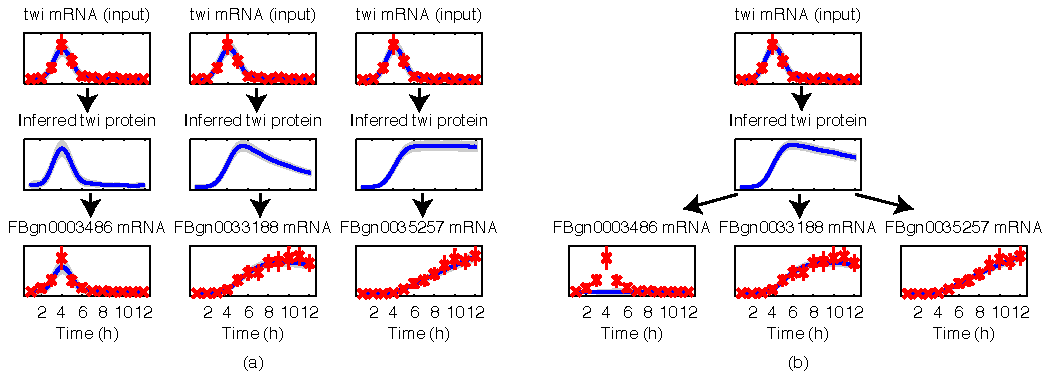
\includegraphics[width=12cm]{../disim_pnas/fig1}
  \caption{Examples of the model fit for two different classes of 
    Gaussian process model fitted to potential targets of the TF Twist~\citep[from][]{Honkela:modelbased10}. (a) Three independent single-target models
    for likely targets. Red marks denote observed expression
    levels from~\cite{Tomancak:systematic02} with 2 s.d.\ error bars.
    The inferred posterior means of the functions are shown in blue
    and the shaded regions denote 2 s.d.\ posterior confidence
    intervals. (b) A joint multiple-target model for
    the same set of target genes as in (a). Note that
    the multiple-target models used in evaluation have more targets
    than the one shown here.\label{fig:gpdisim_models}
}
  %\label{fig:gpdisim_models}
\end{figure}

Figure~\ref{fig:dros_global_evaluation} shows evaluation of the
model-based ranking results using data from a genome-wide
Chromatin-immunoprecipitation (ChIP-chip)
experiment~\citep{Zinzen2009} to determine whether there is evidence
of TF binding within 2000 base-pairs of a putative target. As well as
showing results for the single-target and multiple-target Gaussian
process methods, we also show the performance obtained using evidence
of differential expression in mutant embryos (knock-outs), correlation
with TF expression (correlation) and an alternative maximum likelihood
model-based approach~\citep[quadrature, see][for
details]{Honkela:modelbased10}. In the global validation we score all
genes showing significant variability in the expression data. In the
focused evaluation we only consider genes with annotated expression in
mesoderm or muscle tissue according to the {\em in situ} hybridization
data~\citep{Tomancak:systematic02}.

\begin{figure*}[tb]
  \centering
  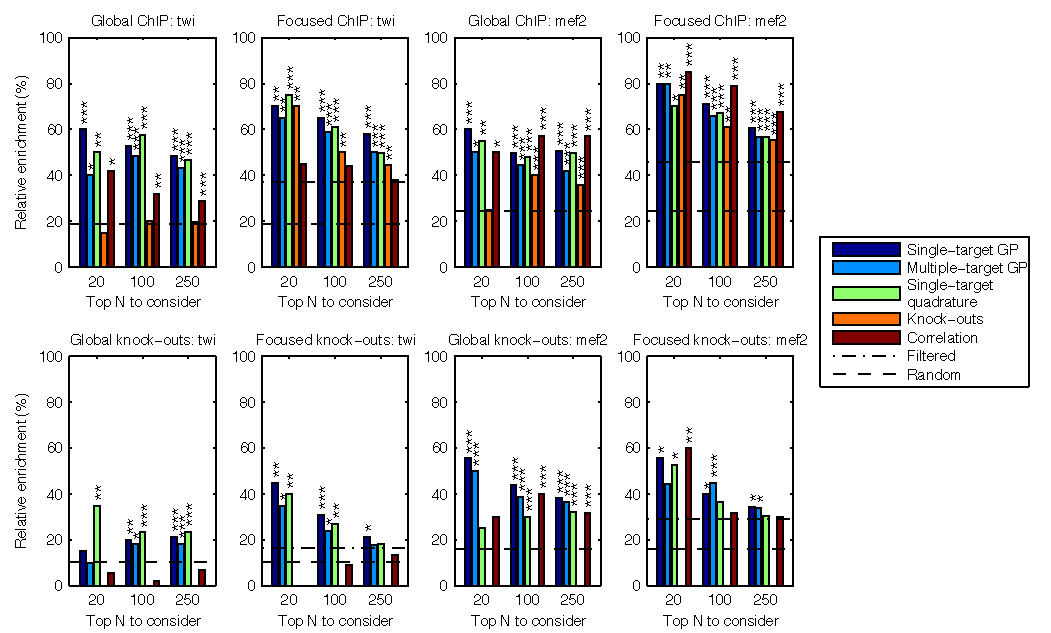
\includegraphics[width=12cm]{../disim_pnas/fig3}
  \caption{Evaluation results of different rankings
    \citep[from][]{Honkela:modelbased10} as
    discussed in the text showing the relative frequency of positive
    predictions among $N$ top-ranking targets (``global'' evaluations)
    or among $N$ top genes
    with annotated expression in mesoderm or muscle tissue
    (``focused'' evaluations).
    The dashed line
    denotes the frequency in the full population and the dash-dot
    line within the population considered in focused evaluation.
    The first row shows the frequency of targets with ChIP-chip
    binding within 2000 base pairs of the gene
    while the second row shows the frequency of
    predicted targets with significant differential
    expression in TF knock-outs.
    $p$-values of results significantly different from random are
    denoted by `***': $p <
    0.001$, `**': $p < 0.01$, `*': $p < 0.05$.
    Comparison to knock-out ranking is obviously omitted for knock-out
    validation. \label{fig:dros_global_evaluation}
  }
 % \label{fig:dros_global_evaluation}
\end{figure*}

We find that the model-based approach provides a significant advantage
over the simpler correlation-based approach for Twist, whose targets
display a diverse range of temporal profiles
(Figure~\ref{fig:gpdisim_models}). For Mef2 the correlation-based
approach works well. We observe that most of the predicted Mef2
targets have profiles very similar to Mef2 itself, in which case the
model-based approach would not be expected to provide an
advantage. The single-target Gaussian process approach is found to
out-perform other methods in most cases~\citep{Honkela:modelbased10}.


\section{Multiple Tanscription Factors}

The models discussed in previous sections are based on the idealized
assumption that the gene regulation process is driven by a single
trascription factor. However, gene regulation in complex biological
systems can involve several TFs.  More precisely, to initiate
trascription of a gene, multiple TFs may be required to simultaneously
bind the related DNA sequence. Thus, in order to take into account the
effect of multiple TFs, we need to generalize the basic single-TF
model described previously. Furthermore, to deal with the
non-negativity of the mRNA and protein TF functions, along with
saturation effects that are naturally encountered in their dynamics,
it is essential to assume biologically plausible non-linearities.
   
The basic single-TF ODE model from Equation 
(\ref{eq:differentialEquation}) can be generalized
to include multiple TFs according to  
\begin{equation}
\diff{\mrnaConcentration_j(t)}{t} = \basalRate_j + 
\sensitivity_j G
\left(\tfConcentration_1(t),\ldots,\tfConcentration_I(t);
  \bfw_j, w_{j0}\right) -\decayRate_j \mrnaConcentration_j(t), \label{eq:multipleTFtranscription}
\end{equation}
where $\tfConcentration_i(t)$, $i=1,\ldots,I$, are the TF protein
functions.  The function $G(\cdot)$ represents a non-linear response
that allows the TFs to competitively or co-operatively activate or
repress the transcription. A reasonable assumption for this non-linear
response is to follow a sigmoidal form, similarly to the
Michaelis-Menten and hill-climbing functions used in single input
motifs \citep{Alon:systems06}. For instance, we can choose
\begin{equation} 
G(\tfConcentration_1(t),\ldots,\tfConcentration_I(t); \bfw_j, w_{j0})
= \frac{1}{1 + e^{-w_{j0}  - \sum_{i=1}^I w_{ji} \log \tfConcentration_i(t)}},
\label{eq:multipleTFhillFun}
\end{equation}
which is the standard sigmoid function that takes values in $[0,1]$
and recieves as inputs the logarithm of the TF activities.  Here,
$w_{j0}$ is a real-valued bias parameter and the $I$-dimensional
real-valued vector $\bfw_j = [w_{j1} \ldots w_{jI}]^T$ represents the
interaction weights between the $j^{\text{th}}$ target gene and the
$I$ TFs. These parameters quantify the strength of the network links
between TFs and genes in the underlying regulatory network.
Specifically, when $w_{ji}=0$ the link between the $j^{\text{th}}$
gene and the $i^{\text{th}}$ TF is absent while when $w_{ji}$ is
negative or positive the TF acts as a repressor or activator
respectively.  Notice that by estimating the values of the interaction
weights, we can infer the network links between TFs and genes. This
can lead to a very flexible framework for target identification which
generalizes the method described in section \ref{sec:targetRanking}.

The multiple TF model can contain a much larger number of unknown
parameters and unobserved protein functions compared to the single
input motif model. Given the scarcity of the data, it is therefore
essential that inference is carried out by a fully Bayesian approach
using Markov chain Monte Carlo (MCMC).  This poses significant
computational challenges since we need to infer via sampling all the
unknown quantities which are the protein functions and the remaining
model parameters.  We have developed an MCMC approach that infers the
TF profiles from a small set of training data, associated with a
moderate-sized network, and then it performs target identification at
a genome-wide scale.
%b yfollowing the framework of section \ref{sec:targetRanking}. 
This Bayesian approach is based on placing 
GP priors on the logged TF concentrations and suitable priors on the
remaining model parameters (i.e.\ interaction weights and kinetic parameters) 
and then simulate from the posterior distribution  
by applying suitable Metropolis-Hastings updates.     


 

\begin{figure}
\begin{center}
\begin{tabular}{ccc}
      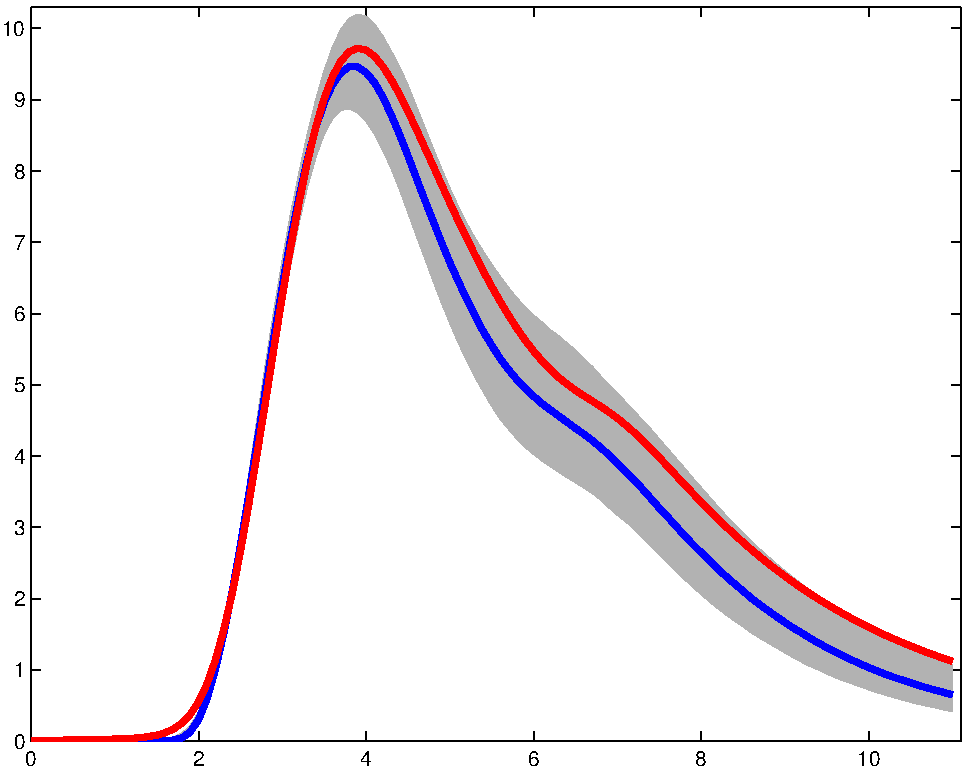
\includegraphics[width=0.3\textwidth]{../diagrams/toyMarch25MCMC19-Sep-2010logOnePlusExpgenHillTFproteins_Rep1TF1} &
      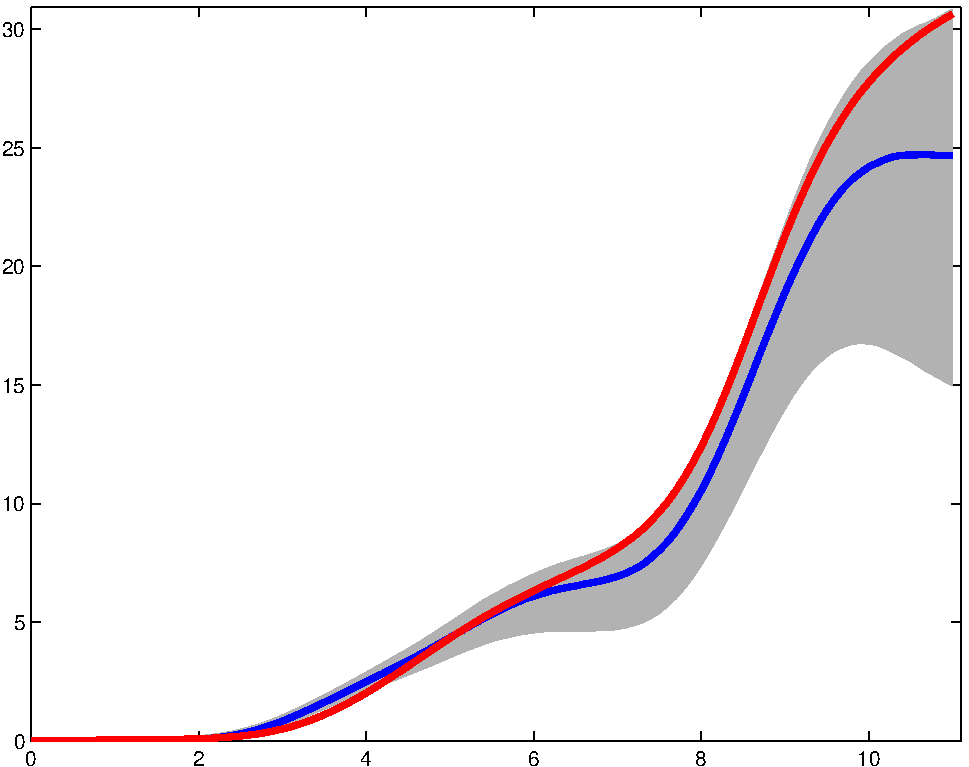
\includegraphics[width=0.3\textwidth]{../diagrams/toyMarch25MCMC19-Sep-2010logOnePlusExpgenHillTFproteins_Rep1TF2} &      
      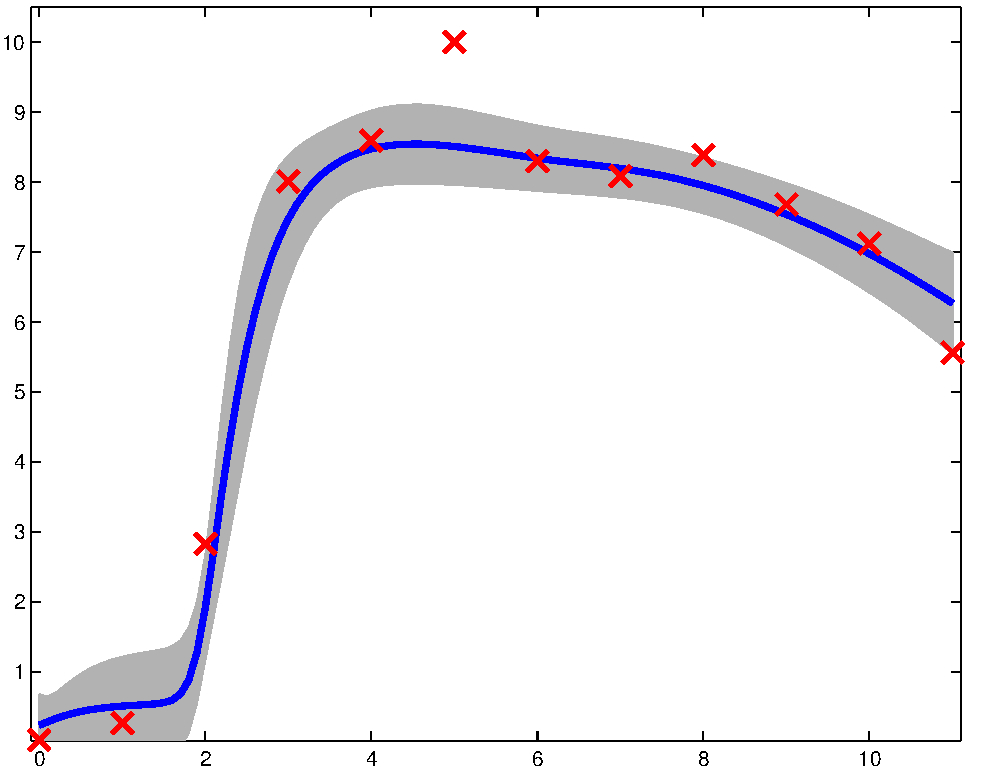
\includegraphics[width=0.3\textwidth]{../diagrams/toyMarch25MCMC19-Sep-2010logOnePlusExpgenHillReplica1GENEmRNA17}\\ 
      (a) & (b) & (c) \\
      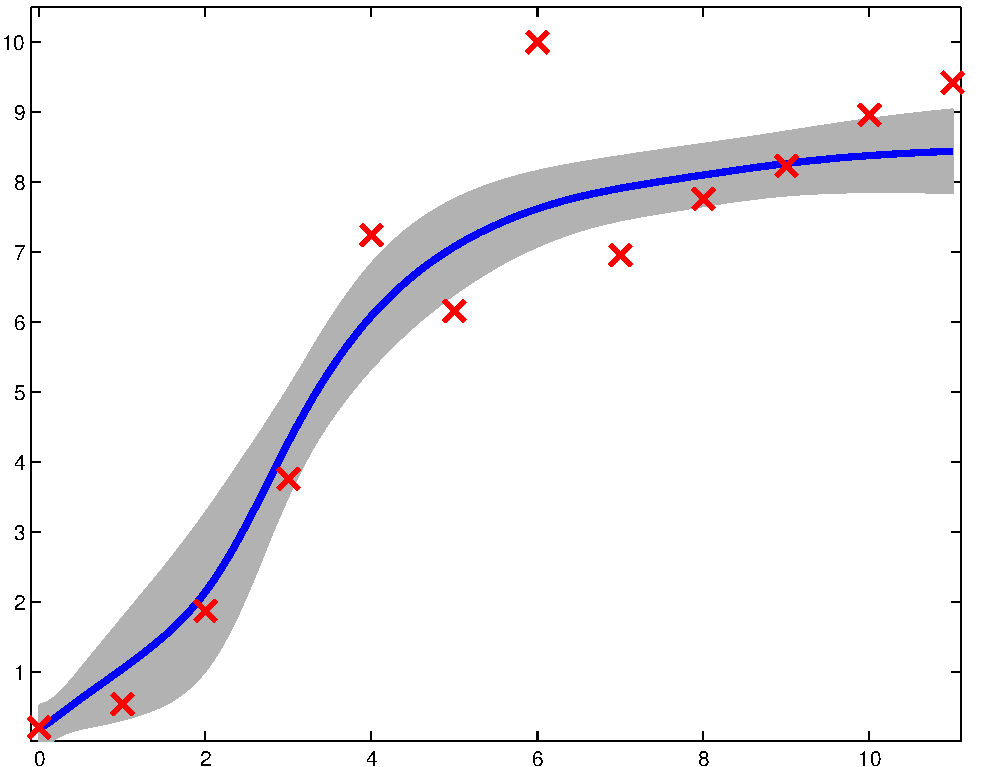
\includegraphics[width=0.3\textwidth]{../diagrams/toyMarch25MCMC19-Sep-2010logOnePlusExpgenHillReplica1GENEmRNA5} &
      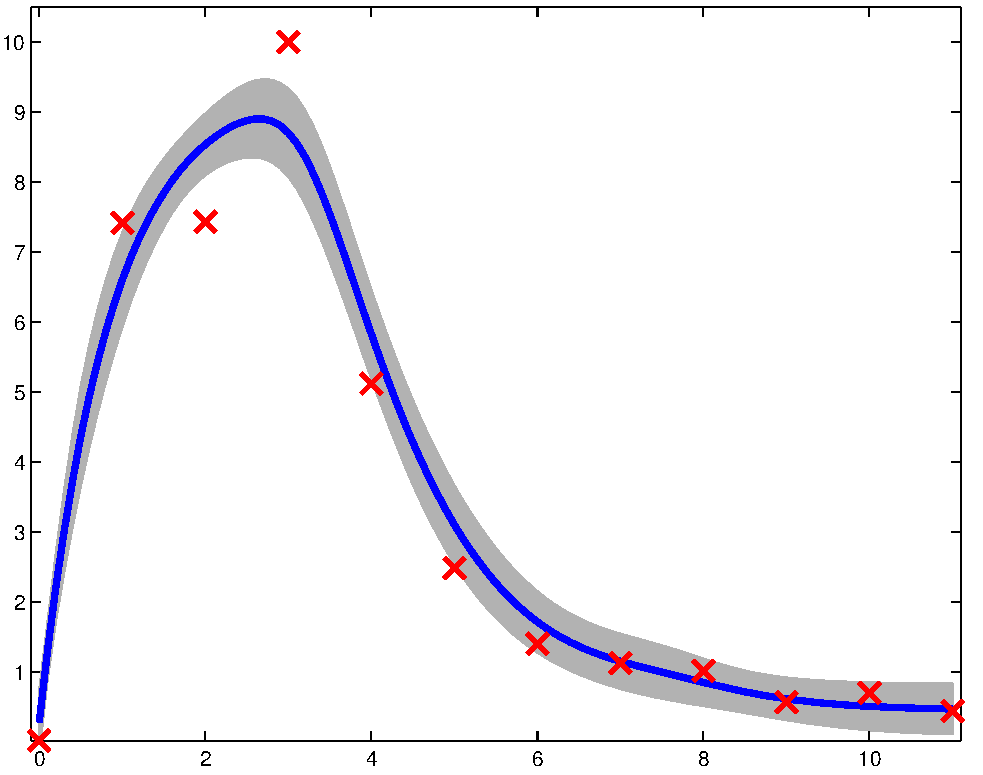
\includegraphics[width=0.3\textwidth]{../diagrams/toyMarch25MCMC19-Sep-2010logOnePlusExpgenHillReplica1GENEmRNA16} &      
      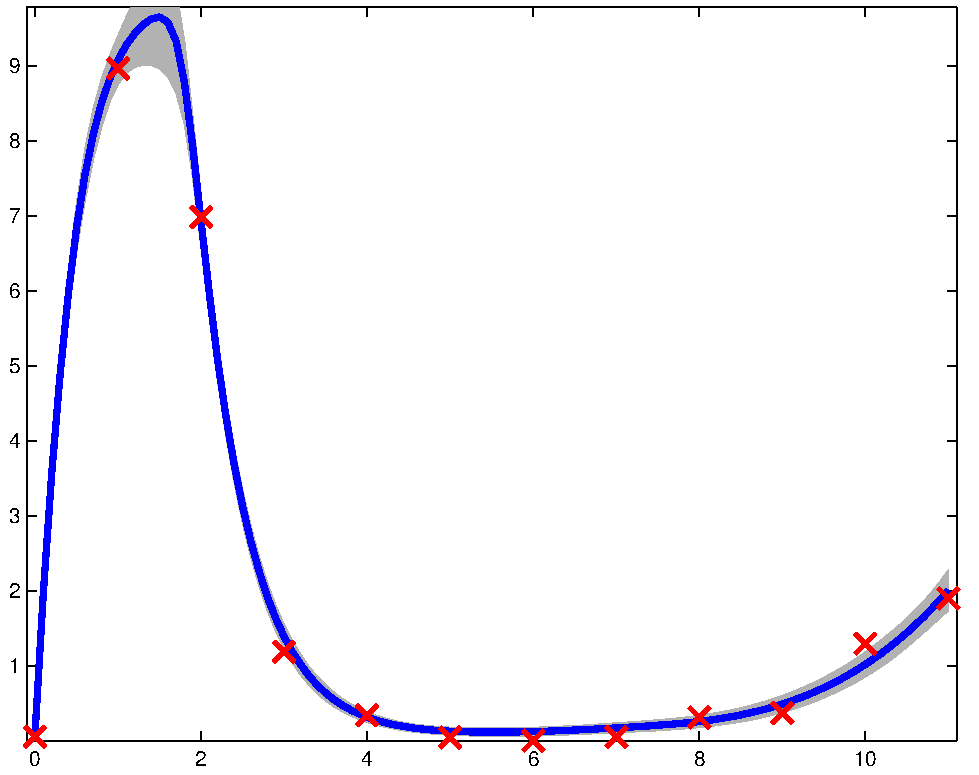
\includegraphics[width=0.3\textwidth]{../diagrams/toyMarch25MCMC19-Sep-2010logOnePlusExpgenHillReplica2GENEmRNA10} \\
      (d) & (e) & (f)
 \end{tabular} 
\end{center}
 \caption{Panels (a) and (b) show the inferred TFs. The estimated
   means are plotted as the blue solid lines and the shaded areas 
   represent $95\%$ uncertainty around the estimated means. 
   The red solid lines show the ground-truth TFs that generated the
   data. 
    Panels (c)-(f) show several examples of how the multiple TF
    model predicts gene mRNA functions. The red crosses denote
    observed measurements, while blue lines and shaded areas represented 
    noisy-free (without adding the observation noise from the likelihood) 
    Bayesian model predictions of the mRNA functions. %All these examples are taken from the
    %training set of the $20$ genes.  
  }\label{fig:toyMultipleTFsFitting}
\end{figure}


 \begin{figure}
  \begin{center}
      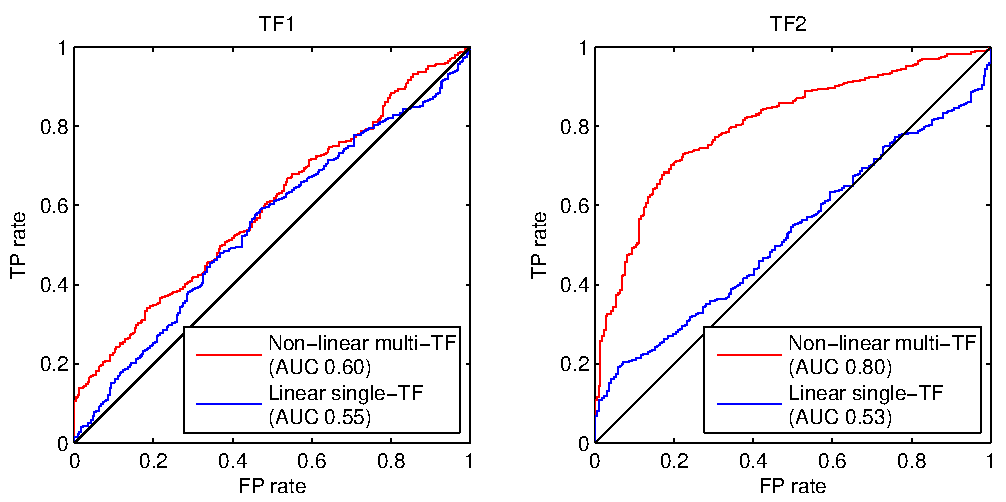
\includegraphics[width=0.8\textwidth]{../diagrams/dros_toy_evaluation.pdf}
\end{center}
\caption{ROC curves for predicting the network connections in the
  synthetic data. The left panel shows the performance when predicting
  the first TF, while the right panel shows performance for predicting
  the second TF.  Red curves show the results by using the multiple TF
  model and blue lines the results by using the linear single-TF
  model.  In both plots, random prediction is represented by the
  diagonal black line.}\label{fig:toyMultipleTFsROCs}
\end{figure}

When observations of the TF mRNAs are available, the above framework
can be combined with the protein translation ODE model presented in
section \ref{sec:targetRanking}.  This can further facilitate the
estimation of the TF profiles and resolve identifiability problems
caused by the scarcity of the data and experimental conditions.


We applied the multiple TF dynamical model to an artifical dataset
consisting of time-series mRNA mesearuments associated with $1000$
genes and two TFs. The network links between TFs and genes are unknown
apart from a small set of $20$ genes which are assumed to have known
connections. This small set of genes is used to infer the TF
concentration functions. Figure \ref{fig:toyMultipleTFsFitting}(a) and
(b) show the inferred TF profiles where blue lines represent the
inferred means, shaded areas represent $95\%$ uncertainty and the red
lines are the actual profiles that generated the data. Figure
\ref{fig:toyMultipleTFsFitting}(c)-(f) give several examples on how
the model fits the mRNA expression data.  Specifically, the panel in
(c) shows a gene that is activated only by the first TF while the
second TF is inactive.  Panel (d) and (e) show two genes that are
regulated (activated in (d) and repressed in (e)) only by the second
TF.  The last panel (f) shows a gene that is jointly regulated by the
two TFs so that it is repressed by the first TF and activated by the
second one.  Figure \ref{fig:toyMultipleTFsROCs} shows ROC curves of
predictive performance for identifying the network links between the
two TFs and the $980$ test genes.  The performance of a linear
single-TF model is also displayed and is clearly inferior to the
performance of the multiple TF model.


\section{Conclusion}

The difficulty of measuring every biochemical species involved in
cellular interaction networks will mean that we will often be faced
with the problem of missing functions. In this chapter we have
reviewed an elegant approach to dealing with such missing functions,
we started with parameteric generalized linear models for dealing with
the missing functions, and extended them through Bayesian treatments
and considering the limit of infinite basis functions to arrive at
sGaussian process models. We reviewed a simple model of transcription
and translation and showed how it can be used to rank putative targets
of transcription factors. The Gaussian process framework provides an
elegant framework for analytically dealing with missing functions if
the differential equation responds in a linear way to the driving
function. However, if we consider nonlinear responses, which we must
necessarily do if we wish to constrain the concentration of the
missing functions to be positive, the analytic approach is no longer
tractable. We reviewed an efficient sampling based approach that
allows us to consider non linear responses and can be applied to the
situation where there are multiple transcription factors regulating
the targets of interest. Both approaches can be applied for genomewide
ranking of putative targets.xs Together these approaches present a
powerful set of diagnostic tools for unravelling the transcriptional
interactions that underpin a biological time series.xs


\bibliographystyle{plainnat}
\bibliography{lawrence,other,zbooks}
  

\end{document}














